\documentclass{article}
\usepackage[utf8]{inputenc}
\usepackage{biblatex} %Imports biblatex package
\addbibresource{sample.bib} %Import the bibliography file

\title{Spring 2024 CS4641/CS7641 Homework 1}
\author{Dr. Mahdi Roozbahani}
\date{Deadline: Friday, February 9th, 11:59 pm EST}
\addtolength{\oddsidemargin}{-.875in}
\addtolength{\evensidemargin}{-.875in}
\addtolength{\textwidth}{1.75in}

\addtolength{\topmargin}{-.875in}
\addtolength{\textheight}{1.75in}
\usepackage{graphicx}
\usepackage{amsmath}
\usepackage{array}
\usepackage{amssymb}
\usepackage{enumitem}
\usepackage{hyperref}
\usepackage{bbold}
\usepackage{diagbox}
\usepackage{multirow}

%new
\usepackage{listings}


\hypersetup{
    colorlinks=true,
    linkcolor=blue,
    filecolor=magenta,      
    urlcolor=cyan,
    pdftitle={Sharelatex Example},
    pdfpagemode=FullScreen,
}

\begin{document}
\maketitle
\begin{itemize}
    \item No unapproved extension of the deadline is allowed. For late submissions, please refer to the course website.
    \item Discussion is encouraged on Ed as part of the Q/A. However, all assignments should be done individually.
    \item \color{red}Plagiarism is a \textbf{serious offense}. You are responsible for completing your own work. You are not allowed to copy and paste, or paraphrase, or submit materials created or published by others, as if you created the materials. All materials submitted must be your own. This also means you may not submit work created by generative models as your own.\color{black}
    \item \color{red}All incidents of suspected dishonesty, plagiarism, or violations of the Georgia Tech Honor Code will be subject to the institute’s Academic Integrity procedures. If we observe any (even small) similarities/plagiarisms detected by Gradescope or our TAs, \textbf{WE WILL DIRECTLY REPORT ALL CASES TO OSI}, which may, unfortunately, lead to a very harsh outcome. \textbf{Consequences can be severe, e.g., academic probation or dismissal, grade penalties, a 0 grade for assignments concerned, and prohibition from withdrawing from the class}.
\end{itemize}

\section*{Instructions}
\begin{itemize}
    \item We will be using Gradescope for submission and grading of assignments. 
    \item \textbf{Unless a question explicitly states that no work is required to be shown, you must provide an explanation, justification, or calculation for your answer.} Basic arithmetic can be combined (it does not need to each have its own step); your work should be at a level of detail that a TA can follow it.
    \item Your write-up must be submitted in PDF form, you may use either Latex,  markdown, or any word processing software. \color{red}We will \textbf{NOT} accept handwritten work. \color{black}Make sure that your work is formatted correctly, for example submit $\sum_{i=0} x_i$ instead of \text{sum\_\{i=0\} x\_i}. 
    \item \textbf{A useful video tutorial on LaTeX has been created by our TA team} and can be found \href{https://www.dropbox.com/s/wywx114wtfoweru/Latex\%20Tutorial.mp4?dl=0}{here} and an Overleaf document with the commands can be found \href{https://www.overleaf.com/read/yjxbshkffvkm}{here}.

    % Possibly change
    \item When submitting your assignment on Gradescope, \textbf{you are required to correctly map pages of your PDF to each question/ subquestion to reflect where they appear.}  Improperly mapped questions will not be graded correctly.
    \item All assignments should be done individually, each student must write up and submit their own answers.
    \item \color{red}\textbf{Graduate Students}\color{black}: You are required to complete any sections marked as Bonus for Undergrads
\end{itemize}
\newpage

\section*{Point Distribution}
\subsection*{Q1: Linear Algebra [38pts]}
\begin{itemize}
    \item 1.1 Determinant and Inverse of a Matrix [15pts]
    \item 1.2 Characteristic Equation [8pts]
    \item 1.3 Eigenvalues and Eigenvectors [15pts]
\end{itemize}
\subsection*{Q2: Expectation, Co-variance and Statistical Independence [9pts]}
\begin{itemize}
    \item 2.1 Covariance [5pts]
    \item 2.2 Correlation [4pts]
\end{itemize}
\subsection*{Q3: Optimization [15pts: 15pts + 2\% Bonus for All]}
\subsection*{Q4: Maximum Likelihood [25pts: 10pts + 15 pts Grad/6\% Bonus for Undergrads]}
\begin{itemize}
    \item 4.1 Discrete Example [10pts]
    \item 4.2 Poisson Distribution [15pts Grad / 6\% Bonus for Undergrads]
\end{itemize}
\subsection*{Q5: Information Theory [32pts]}
\begin{itemize}
    \item 5.1 Marginal Distribution [6pts]
    \item 5.2 Mutual Information and Entropy [16pts]
    \item 5.3 Entropy Proofs [10pts]
\end{itemize}
\subsection*{Q6: Ethical Implications on Decision-Making [5 pts]}
\subsection*{Q7: Programming [5pts]}
\subsection*{Q8: Bonus for All [8\%]}
\subsection*{Points Totals:}
\begin{itemize}
    \item \textbf{Total Base:} 114 pts
    \item \textbf{Total Undergrad Bonus:} 6\%
    \item \textbf{Total Bonus for All:} 10\%
    \item \textbf{Total Possible Assignment Grade (Undergrad):} 116\%
    \item \textbf{Total Possible Assignment Grade (Grad):} 110\%
\end{itemize}

\newpage

\section{Linear Algebra [15pts + 8pts + 15pts]}
\subsection{Determinant and Inverse of Matrix [15pts]}
Given a matrix $M$:
$$M = \begin{bmatrix} 
    2 & 0 & 1 \\ 
    -1 & r & -3 \\
    2 & 5 & -4
\end{bmatrix}$$
\begin{enumerate}[label=(\alph*)]
    \item Calculate the determinant of $\boldsymbol{M}$ in terms of $r$ (calculation process is required). [4pts]
    $$|\boldsymbol{M}| = \text{\textcolor{red}{Start your answer here.}} $$

    \item For what value(s) of $r$ does $\boldsymbol{M}^{-1}$ not exist? Why doesn't $\boldsymbol{M}^{-1}$ exist in this case? What does it mean in terms of rank and singularity for these values of $r$? \textit{This question can be answered in less than 7 lines. } [3pts]
    
    % answer below
    \textcolor{red}{Start your explanation here.} % delete this line after
    % end answer
    
    \item Will all values of $r$ found in part (b) allow for a column (or row) to be expressed as a linear combination of the other columns (or rows)? \textbf{If yes}, provide
    \begin{itemize}
        \item \textbf{either} the linear equation of the second column $\boldsymbol{C_2}$ as a linear combination of the first column $\boldsymbol{C_1}$ and third column $\boldsymbol{C_3}$
        \item \textbf{or} the linear equation of the third row $\boldsymbol{R_3}$ as a linear combination of the first row $\boldsymbol{R_1}$ and second row $\boldsymbol{R_2}$.
        \item (calculation process is \textbf{NOT} required).
    \end{itemize}
    \textbf{If no}, explain why. [3pts]


    % answer below
    \textcolor{red}{Start here: } $C_2 = \frac{a}{b}C_1 + \frac{c}{d}C_3$, or $R_3 = \frac{a}{b}R_1 + \frac{c}{d}R_2$.
    % end answer 
    \item Write down $\boldsymbol{M}^{-1}$ for $r = 0$ (calculation process is \textbf{NOT} required). [2pts]
    % answer below
    $$ M^{-1} = 
    \textcolor{red}{\begin{bmatrix} 
        a & b & c \\ 
        d & e & f \\
        g & h & i
    \end{bmatrix}}$$
    \textcolor{red}{Change the values in the above matrix.}
    % end answer
    \item Find the mathematical equation that describes the relationship between the determinant of $\boldsymbol{M}$ and the determinant of $\boldsymbol{M}^{-1}$. [3pts]
    \par\textbf{NOTE:} It may be helpful to find the determinant of $\boldsymbol{M}$ and $\boldsymbol{M}^{-1}$ for $r = 0$.
    % answer below
    
    % end answer
\end{enumerate}
\newpage



\subsection{Characteristic Equation [8pts]}
Consider the eigenvalue problem: 
$$\boldsymbol{Ax} =\lambda \boldsymbol{x}, \boldsymbol{x} \neq 0$$
where $\boldsymbol{x}$ is a non-zero eigenvector and $\lambda$ is an eigenvalue of $\boldsymbol{A}$. Prove the determinant $|\boldsymbol{A}-\lambda \boldsymbol{I}|= 0$.\\ \\
\textbf{NOTE:} There are many ways to solve this problem. You are allowed to use linear algebra properties as part of your solution. \\
\newpage



\subsection{Eigenvalues and Eigenvectors [5+10pts]}
\subsubsection{Eigenvalues [5pts]}
Given the following matrix $\boldsymbol{A}$, find an expression for the eigenvalues $\lambda$ of $\textbf{\textit{A}}$ in terms of $a$, $b$, and $c$. Express your answer in the form $\lambda =$... [5pts] 

$$\textbf{\textit{A}}=\begin{bmatrix}
    a & b \\
    b & c
\end{bmatrix}$$


\subsubsection{Eigenvectors [10pts]}
Given a matrix $\boldsymbol{A}$:
$$\boldsymbol{A} = \begin{bmatrix} 
    x & 9  \\ 
    4 & x \\
\end{bmatrix}$$
\begin{enumerate}[label=(\alph*)]
    \item Calculate the eigenvalues of $\boldsymbol{A}$ as a function of $x$ (calculation process required). [3pts]
    \item Find the normalized eigenvectors of matrix $\boldsymbol{A}$ (calculation process required). [7pts]
\end{enumerate}

\newpage
\section{Expectation, Co-variance and Statistical Independence [5pts + 4pts]}
\subsection{Covariance [5pts]}
Suppose $X$, $Y$, and $Z$ are three different random variables.
Let $X$ obey a two point Distribution. The probability mass function for $X$ is:
    $$p(x)=\left\{
    \begin{array}{ c l}	
        0.4 & x = c\\
        0.6 & x = -c
    \end{array}\right.$$
where $c$ is a nonzero constant. Let $Y$ obey the Standard Normal (Gaussian) Distribution, which can be written as $Y \sim N(0,1)$. $X$ and $Y$ are statistically independent (i.e. $P(X|Y) = P(X)$). Meanwhile, let $Z = XY$. \\

\noindent Calculate the covariance of $Y$ and $Z$ (i.e. $Cov(Y, Z)$). Do values of $c$ affect the covariance between $Y$ and $Z$? [5pts]

\newpage
\subsection{Correlation Coefficient [4pts]}
Let $X$ and $Y$ be statistically independent random variables with $Var(X) = 3$ and $Var(Y) = 6$. We do not know $E[X]$ or $E[Y]$. Let $Z = 2X + 3Y$ . Calculate the correlation coefficient defined as $\rho(X,Z)=\frac{Cov(X,Z)}{\sqrt{Var(X)Var(Z)}}$. If applicable, please round your answer to 3 decimal places. [4pts]


\newpage
\section{Optimization [15pts + 2\% Bonus for All]}
Optimization problems are related to minimizing a function (usually termed loss, cost or error function) or maximizing a function (such as the likelihood) with respect to some variable $x$. The Karush-Kuhn-Tucker (KKT) conditions are first-order conditions for a solution in nonlinear programming to be optimal, provided that some regularity conditions are satisfied. In this question, you will be solving the following optimization problem:
\begin{align*}
    \min_{x,y} \qquad & f(x,y) = xy-8y \\
    \text{s.t.} \qquad & g_{1}(x,y) = 2x^{2}+y^{2}\leq 20 \\
    & g_{2}(x,y) =  x \leq 1
\end{align*}

\begin{enumerate}[label=(\alph*)]
    \item Write the Lagrange function for the minimization problem. Now change the minimum function to a maximum function (i.e. $\underset{x,y}{max} \;\; f(x,y) = xy - 4x$) and provide the Lagrange function for the maximization problem with the same constraints $g_1$ and $g_2$.  [2pts]
        \par\textbf{NOTE:} The maximization problem is only for part (a).
    \item List the names of all 4 groups of KKT conditions and their corresponding mathematical equations or inequalities for this specific minimization problem. [2pts]
    \item Solve for 4 possibilities formed by each constraint being active or inactive. Do not forget to check the inactive constraints for each point when applicable. Candidate points must satisfy all the conditions mentioned in part b).   [7pts]
    \item List the candidate point(s) (there is at least 1) obtained from part c). Please round answers to 3 decimal points and use that answer for calculations in further parts. This part can be completed in one line per candidate point. [2pts]
    \item Find the \textbf{one} candidate point for which $f(x,y)$ is largest. Check if $L(x,y)$ is concave or convex at this point by using the \href{https://www.khanacademy.org/math/multivariable-calculus/applications-of-multivariable-derivatives/quadratic-approximations/a/the-hessian}{Hessian} in the \href{https://www.khanacademy.org/math/multivariable-calculus/applications-of-multivariable-derivatives/optimizing-multivariable-functions/a/second-partial-derivative-test}{second partial derivative test}.  [2pts]
    \item \textbf{BONUS FOR ALL:} Make a 3D plot of the objective function $f(x,y)$ and constraints $g_1$ and $g_2$ using \href{https://www.math3d.org/}{Math3d}. Mark the minimum candidate point and include a screenshot of your plot. Briefly explain why your plot makes sense in one sentence. Although this is bonus, this is \textbf{VERY HELPFUL} in understanding what was accomplished in this problem. [2\%]
    \par\textbf{NOTE:} Use an explicit surface for the objective function, implicit surfaces for the constraints, and a point for the minimum candidate point. \\
\end{enumerate}

\noindent\textbf{HINT:} Read the Example\_optimization\_problem.pdf in Canvas Files for HW1 to see an example with some explanations. \\
\noindent\textbf{HINT:} Click \href{https://www.youtube.com/watch?v=TqN-8fxYUYY}{here} for a video explaining the intuition behind KKT problems.\\
\noindent\textbf{HINT:} Click \href{https://www.youtube.com/watch?v=TqN-8fxYUYY}{here} for an example maximization problem. It's recommended to only watch up until 23:14. \\
\noindent\textbf{HINT:} Click \href{https://en.wikipedia.org/wiki/Karush-Kuhn-Tucker_conditions#Nonlinear_optimization_problem}{here} to determine how to set up the problem for minimization in part (a) and for KKT conditions in part (b).\\



\newpage

\section{Maximum Likelihood [10pts + 15pts Grads / 6\% Bonus for Undergrads]}
\subsection{Discrete Example [10pts]}
Mastermind Mahdi decides to give a challenge to his students for their MLE Final. He provides a spinner with 12 sections, each numbered 1 through 12. The students can change the sizes of each section, meaning that they can select the probability the spinner lands on a certain section. Mahdi then proposes that the students will get a 100 on their final if they can spin the spinner 12 times such that it doesn't land on section 1 during the first 11 spins and lands on section 1 on the 12th spin. If the probability of the spinner landing on section 1 is $\theta$, what value of $\theta$ should the students select to most likely ensure they get a 100 on their final? Use your knowledge of Maximum Likelihood Estimation to get a 100 on the final. \\\\\textbf{NOTE: } \textbf{You must specify the log-likelihood function and use MLE to solve this problem for full credit.} You may assume that the log-likelihood function is concave for this question \\\\

\begin{center}
    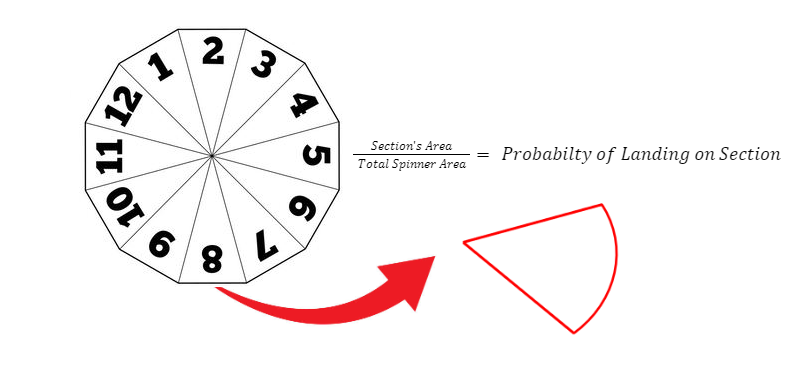
\includegraphics[origin=c,scale=.5]{spinner.PNG} 
\end{center}


\newpage

\subsection{Poisson distribution [15 pts Grad / 6\% Bonus for Undergrads]}
The Poisson distribution is defined as:
$$P(X=k)=\frac{\lambda^k e^{-\lambda}}{k!} (k=0,1,2,...).$$
\begin{enumerate}[label=(\alph*)]
    \item Let $X_1 \sim Poisson(\lambda)$, and $x_1$ be an observed value of $X_1$. What is the likelihood given $\lambda$? [2 pts / 0.8\%]
    \item Now, assume we are given $n$ such values. Let $(X_1, ...,X_n)\sim Poisson(\lambda)$ where $X_1, ...,X_n$ are i.i.d. random variables, and $x_1,...,x_n$ be observed values of $X_1, ...,X_n$. What is the likelihood of this data given $\lambda$? You may leave your answer in product form. [3 pts / 1.2\%]
    \item What is the maximum likelihood estimator of $\lambda$? [10 pts / 4\%]
\end{enumerate}

\newpage

\section{Information Theory [6pts + 16pts + 10pts]}
\subsection{Marginal Distribution [6pts]}

Suppose the joint probability distribution of two binary random variables $X$ and $Y$ are given as follows. $X$ are the rows, and $Y$ are the columns.
$$\renewcommand*{\arraystretch}{1.3}
\begin{tabular}{|c|c|c|}
    \hline 
    \diagbox{X}{Y} & {0} & {1} \\ 
    \hline 0 & {$\frac{4}{12}$} & {$\frac{1}{12}$} \\ 
    \hline 
    1 & {$\frac{2}{12}$} & {$\frac{5}{12}$} \\ 
    \hline
\end{tabular}$$

\begin{enumerate}[label=(\alph*)]
    \item Show the marginal distribution of $X$ and $Y$, respectively. [3pts]
    \item Find mutual information $I(X,Y)$ for the joint probability distribution in the previous question to at least 5 decimal places (please use base 2 to compute logarithm) [3pts]
\end{enumerate}

\newpage

\subsection{Mutual Information and Entropy [16pts]}
% temp link until something more permanent (perhaps on canvas)
A recent study has shown symptomatic infections are responsible for higher transmission rates. Using the \href{https://docs.google.com/spreadsheets/d/1KYade9n4Gh34GMgdJAQt3qHVxFx48jqAXX4kNu4XrZQ/edit?usp=sharing}{data} collected from positively tested patients, we wish to determine which feature(s) have the greatest impact on whether or not some will present with symptoms. To do this, we will compute the entropies, conditional entropies, and mutual information of select features. Please use base 2 when computing logarithms.
\begin{table}[h]
\centering
\begin{tabular}{|c|c|c|c|c|c|}
\hline
\multicolumn{1}{|c|}{\multirow{2}{*}{\textbf{ID}}} & \multicolumn{1}{c|}{\multirow{2}{*}{\textbf{\begin{tabular}[c]{@{}c@{}}Vaccine Doses \\ ($X_1$)\end{tabular}}}} & \multicolumn{1}{c|}{\multirow{2}{*}{\textbf{\begin{tabular}[c]{@{}c@{}}Wears Mask? \\ ($X_2$)\end{tabular}}}} & \multicolumn{1}{c|}{\multirow{2}{*}{\textbf{\begin{tabular}[c]{@{}c@{}}Underlying \\ Conditions ($X_3$)\end{tabular}}}} & \multicolumn{1}{c|}{\multirow{2}{*}{\textbf{\begin{tabular}[c]{@{}c@{}}Symptomatic \\ ($Y$)\end{tabular}}}} \\
\multicolumn{1}{|c|}{} & \multicolumn{1}{c|}{} & \multicolumn{1}{c|}{} & \multicolumn{1}{c|}{} & \multicolumn{1}{c|}{} \\ \hline \hline
1 & M & T & T & T \\ \hline
2 & M & F & F & T \\ \hline
3 & L & F & T & F \\ \hline
4 & M & T & F & T \\ \hline
5 & M & F & T & T \\ \hline
6 & M & T & F & F \\ \hline
7 & H & F & T & T \\ \hline
8 & L & T & F & F \\ \hline
9 & L & F & F & T \\ \hline
10 & L &F & F & T \\ \hline
\end{tabular}
\caption{Vaccine Doses: \{(H) booster, (M) 2 doses, (L) 1 dose, (T) True, (F) False\}}
\label{table:1}
\end{table}

\begin{enumerate}[label=(\alph*)]
    \item Find entropy $H(Y)$ to at least 3 decimal places. [3pts]
    \item Find conditional entropy $H(Y|X_1)$ and $H(Y|X_3)$ to at least 3 decimal places. [7pts]
    \item Find mutual information $I(X_1, Y)$ and $I(X_3, Y)$ to at least 3 decimal places and determine which one ($X_1$ or $X_3$) is more informative. [3pts]
    \item Find joint entropy $H(Y, X_2)$ to at least 3 decimal places. [3pts]
\end{enumerate}

\newpage

\subsection{Entropy Proofs [10pts]}

\begin{enumerate}[label=(\alph*)]
    \item Write the discrete case mathematical definition for $H(X|Y)$ and $H(X)$. [3pts]
    \item \textbf{Using the mathematical definition of $H(X)$ and $H(X|Y)$ from part (a)}, prove that $I(X,Y) = 0$ if $X$ and $Y$ are statistically independent. (Note: you must provide a mathematical proof and cannot use the visualization shown in class \href{https://mahdi-roozbahani.github.io/CS46417641-summer2022/other/CEandMI_Illustration.jpg}{found here}. You may use any theorem/ proof from the slides without having to re-prove it). [7pts] \\
    \newline
    \color{red}{\textbf{Start from: $I(X,Y) = H(X)-H(X|Y)$}}
\end{enumerate}

\newpage

\section{Ethical Implications on Decision-Making [5 pts]}
\subsection*{Real-world Implications}
Loan eligibility determines who can receive a loan, typically based on financial history and demographics. It is a difficult problem, and often uses algorithms to make loan decisions. Often, this can result in reinforcing inequality and bias \cite{oneil}.\\

Suppose we're using a matrix to represent the attributes of individuals for loan approval. Each attribute (like income, credit score, years of employment, etc.) constitutes a column in our matrix. Here's a hypothetical toy example:\\\\
\begin{tabular}{1 | c c c c}
    \text{} & \text{Annual Income} & \text{Debt-to-Income Ratio} & \text{Employment History (years)} & \text{Credit Score} \\
    \hline
    \text{Candidate 1} & 50,000 & 0.2 & 5 & 700 \\
    \text{Candidate 2} & 51,000 & 0.21 & 5.1 & 710 \\
    \text{Candidate 3} & 45,000 & 0.19 & 4.9 & 690 \\
    \text{Candidate 4} & 100,000 & 0.05 & 10 & 780 \\
\end{tabular}
\\
\\
\\
One algorithm used to predict credit score is linear regression, formulated as $\mathbf{y}=\mathbf{x}\mathbf{A}$. $\mathbf{y}$ are the target variables, $\mathbf{x}$ are the input features, and $\mathbf{A}$ is a matrix trained with an existing dataset. Training data $(\mathbf{x_D}, \mathbf{y_D})$ are taken from the training dataset $D$, $(\mathbf{x_D}, \mathbf{y_D}) \in D$. If $\mathbf{x_D}$ is linearly independent, $\mathbf{A}$ can be trained by simply inverting $\mathbf{x_D}$:
\begin{align*}
    \mathbf{y_D} &= \mathbf{x_D}\mathbf{A} \\
    \mathbf{x_D}^{-1} \mathbf{y_D} &= \mathbf{A}
\end{align*}

The original equation can be rewritten as:
\begin{align*}
    \mathbf{y} &= \mathbf{x}\mathbf{A} \\
    &= \mathbf{x}\mathbf{x_D}^{-1}\mathbf{y_D}
\end{align*}

Problems arise when the training data is close to linearly dependent. Recall that one way to invert a matrix is $\mathbf{A}^{-1} = \frac{1}{\det(\mathbf{A})} \text{adj}(\mathbf{A})$. As $\mathbf{A}$ becomes more linearly dependent and $\det(\mathbf{A}) \rightarrow 0$, $||\mathbf{A}^{-1}||$ can become so large it causes numerical errors. Rewriting the original equation:
\begin{align*}
    \mathbf{y} &= \mathbf{x} \mathbf{x_D}^{-1}\mathbf{y_D} \\
    &= \frac{1}{\det(\mathbf{x_D})} \mathbf{x} \: \text{adj}(\mathbf{x_D}) \mathbf{y_D}
\end{align*}

The errors caused by $\det(\mathbf{x_D}) \rightarrow 0$ propagate to $\mathbf{y}$, causing predictions to be wildly inaccurate anywhere outside of the original training set.

\subsection*{Practical Implications}

\begin{enumerate}
    \item Instability: With a small determinant, minor variations in the attributes can lead to significant variations in the results. So, a small difference in income might result in a disproportionate change in loan eligibility.
    \item Poor Generalization: If the matrix is based on data with limited variation (like our small community example), it's essentially trained on a very narrow subset of potential applicants. If someone from outside this narrow subset applies (e.g., a person with a 2-year employment but a \$70,000 income), the system may not process their application fairly or accurately because it's unfamiliar with such profiles.
\end{enumerate}

\noindent
\textbf{Given that a matrix used for determining loan approvals has a determinant close to zero due to limited variation in applicants' attributes:} \\
\textit{Which of the following implications might this have on the decision-making process? Choose as all options that apply. Use "textbf\{\}" to select your answer.}
\begin{enumerate}[label=\Alph*)]
    \item It ensures a more uniform scoring system since most applicants have similar attributes.
    \item It can lead to unpredictable scores, where tiny variations in attributes yield vastly different outcomes.
    \item The system is more resilient to errors because of the limited attribute variation.
    \item It might not generalize well to broader populations, potentially leading to biases when applied to more diverse applicant groups.
\end{enumerate}

\newpage

\section{Programming [5 pts]}
See the Programming subfolder in Canvas.
\newpage

\section{Bonus for All [8\%]}
\begin{enumerate}[label=(\alph*)]
    \item Let $X$, $Y$ be \textbf{two statistically independent} $N(0, 1)$ random variables, and $P$, $Q$ be random variables defined as: 
    \begin{align*}
        P &= 3X + 2XY^2 \\
        Q &= X
    \end{align*}
    Calculate the variance $Var(P + Q)$. \textit{(This question may take substantial work to support, e.g. 25 to 30 lines)} [4\%]
    
    \textbf{HINT:} The following equality may be useful: $Var(XY) = E[X^2Y^2] - [E(XY)]^2$ \\
    \textbf{HINT:} $E[Y^4] = \int_{-\infty}^{\infty}y^4 f_Y(y)dy$ where $f_Y(y)$ is the probability density function of $Y$ (Wolfram alpha calculator or other similar calculators can be used) \\
    \textbf{HINT:} $Var(P + Q) = Var(P) + Var(Q) + 2Cov(P, Q)$ may be a good starting point.
    
    \item Suppose that $X$ and $Y$ have joint pdf given by:
    $$f_{X,Y}(x,y)=\left\{
    \begin{aligned}
        &\frac{x}{3}e^{-y} & 0 \leq x \leq 3, y \geq 0 \\
        &0 & otherwise\\
    \end{aligned}\right.$$
    What are the marginal probability density functions for $X$ and  $Y$? \textit{(It is possible to thoroughly support your answer to this question in 8 to 10 lines)} [2\%]

    \begin{align*}
        f_X(x) &= \text{\textcolor{red}{Start your answer here.}} \\
    \end{align*}

    \item A person decides to toss a biased coin with $P(heads)=0.1$ repeatedly until he gets a head. He will make at most 5 tosses. Let the random variable $Y$ denote the number of heads. Find the probability distribution of $Y$. Then, find the variance of $Y$. \textit{(It is possible to thoroughly support your answer to this question in 5 to 10 lines)} [2\%]    
\end{enumerate}

\printbibliography

\end{document}
